\documentclass[]{tufte-handout}
\usepackage{amsmath,amssymb,amsthm,color}
\usepackage{multirow}
\usepackage{booktabs}
\usepackage[pdftex]{graphicx}

  
\title{COMP 161 - Lecture Notes - 05 - The Compiler}


\begin{document} 
\maketitle

\begin{abstract}
In these notes we talk about compiling our multi-file C++ program in order to check syntax errors, run unit-tests, or build the main executable. After learning the basics of the the GNU Compiler Collection's\sidenote{GCC} C++ compiler \textbf{g++}, we'll look at using \textbf{make} and Makefiles to manage the compilation process.
\end{abstract}

\section{Our Example Program}

We'll be exploring the compilation of a simple four file program developed with our organizational style.  This is a toy program that computes the factorial in several different ways.  The files are as follows:
\begin{enumerate}
\item \textit{factorial.h} \\ The \textsc{header file} for the factorial library.
\item \textit{factorial.cpp} \\ The \textsc{implementation file} for the factorial library.
\item \textit{fact\_test.cpp} \\ The \textsc{unit tests} for the factorial library
\item \textit{lab2\_main.cpp} \\ The \textsc{main procedure} that utilizes that lets you compute the factorial using several different methods.
\end{enumerate}

Our goal is to compile this code for three purposes:
\begin{enumerate}
\item Compile one or more cpp files to a non-executable object file to check for syntax errors.
\item Compile our tests to an executable that lets us run and evaluate unit tests.
\item Compile the main procedure and program to an executable version of our program.  
\end{enumerate}
Before we tease out commands for these tasks, let's familiarize ourselves with the basic capabilities of the compiler and the process by which code turns in to an executable.

\section{The Compilation Process}

Our compiler carries out a four stage process\sidenote{the verbose option, -v, shows you everything the compiler does. try it sometime}: 
\begin{enumerate}
\item \textsc{Preprocessor} 
\item \textsc{Compiler} 
\item \textsc{Assembler} 
\item \textsc{Linker} 
\end{enumerate}

The g++ compiler has options which allow you to control how much of this process is carried out\sidenote{\url{http://gcc.gnu.org/onlinedocs/gcc/Overall-Options.html}}.  Absent these options, it will take whatever you give it and attempt to finish the compilation process. So, if you give something that's already been preprocessed, it will attempt to compile, assemble, and link it. If you give something that's gone through the assembler, it will attempt to link it. Now let's look a bit at what each of these stages accomplishes.

\subsection{Preprocessor}

The preprocessor essentially transforms our C++ in to different C++ from it. Perhaps the most important transformation it does is to process all the statements beginning with the \textbf{\#} character. The most notable of these is \textit{\#include}, which more or less tells the preprocessor to copy and paste a header file in to the current file. The preprocessor is also a vital component of our unit testing framework, gTest\sidenote{\url{https://code.google.com/p/googletest/wiki/Primer}}.  The tests we write look like procedures, but are in fact Macros\sidenote{A macro gets expanded into C++ code by the processor}. So, when we write our tests, the preprocessor transforms all of our code into different C++ as directed by the unit testing macros.

The option \textbf{-E} causes the compiler to stop after preprocessing and then print the output to the terminal.  We can use \textit{$>$} to redirect the output from stdout to a a file. To see the what happens to the include directives, we could do.
\begin{verbatim}
g++ factorial.cpp -E > pp_factorial.cpp
\end{verbatim}

For a really drastic transformation, look at what happens to our unit test macros:
\begin{verbatim}
g++ fact_tests.cpp > pp_fact_tests.cpp
\end{verbatim}

We'll almost never have cause to stop after pre-processing, but you should still be aware of this stage and the role it plays in building your program. 

\subsection{Compiler}

The compiler is where the whole system gets it name.  It turns high-level C++ into low level assembly.  We can stop the compiler after it compiles using the \textbf{-S} option. By default, this option produces an assembly code file with the \textit{s} extension but the same name as the file being compiled\sidenote{so we don't need to name the output with -o}. If you want to see some assembly try:
\begin{verbatim}
g++ factorial.cpp -S
\end{verbatim}
To view the assembly code, just open the newly created \textit{factorial.s} with emacs or less. The assembly code is the most accurate representation of what the computer really does when our program is running.  When you're doing supper fine-tuned optimizations or tracking down really nasty bugs, you might have to look at the assembly.  Thankfully, we'll never be in this situation in this class. So, you'll never really have cause to use the -S option.  

\subsection{Assembler}

The assembler takes human readable assembly\sidenote{assuming you know the language} and produces a machine readable \textsc{object file}.   The \textbf{-c} option will produce an object file with the same name as your source file\sidenote{cpp file} but with the \textit{o} extension instead of cpp.  This stage is as far as you can go without a main procedure and the stage we target to run a complete check of the syntax. \textit{We'll compile to object files often.}  

You would use the following command to build an object file for the factorial library.
\begin{verbatim}
g++ factorial.cpp -c
\end{verbatim}

You can open the resultant \textit{factorial.o} with emacs and clearly see that, to the human eye, it's gibberish.  

\subsection{Linker}

The linker stitches together object files and creates an executable.  This means that one\sidenote{and only one!} of the object files must contain a main procedure.  There's no special command to link, just don't use any of the other options. Assuming we used the option \textit{-c} to create \textit{factorial.o} and \textit{lab2\_main.o}, we could build our executable as follows:
\begin{verbatim}
g++ factorial.o lab2_main.o 
\end{verbatim}
By default, the compiler names the executable \textit{a.out}. This is a terrible, terrible name. It is not the least bit descriptive and provides now cues as to the effect and purpose of the program. It also means you can only have a single executable in your current directory.  We want two executable, a main executable and the executable to run our tests. We could use CLI commands to rename files, but the compiler provides an option for naming compilation output files: \textit{-o $<$output-name$>$}.

This command produces an executable named \textit{factorial}.
\begin{verbatim}
g++ factorial.o lab2_main.o -o factorial
\end{verbatim}
Along with the assemble option, we'll use this form of the \textit{g++} often. 

\subsection{Errors and Warnings}

Every part of the compiling process checks for problems. When no problems are found, all of the commands listed above produce no output to the stdout.  Instead they produce files; which is a file \textsc{I/O} side-effect.  More often than not, the compiler will find a problem. In fact, we'll often tell the compiler to more aggressively look for suspicious code and report it back to us as an error or warning.  

When building objects, we'll always use the \textit{-Wall} option to tell the compiler to report warnings about code that could be the cause of problems down the line. We might like to ignore these warnings, but as professionals we're concerned about correct code and so we'll try to address all or most of them as they come up.  To assemble and object file with warnings, we use the following:
\begin{verbatim}
g++ factorial.cpp -c -Wall 
\end{verbatim}

Errors and warnings show up on the CLI. Here's the error you get\sidenote{you \textit{will} see this at some point} when you forget a semi-colon.
\vspace{.1in}
\begin{center}
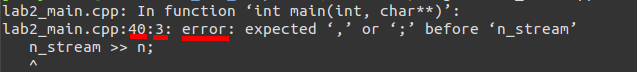
\includegraphics[scale=.5]{compiler-error.png}
\end{center}
\vspace{.1in}
The numbers underlined are the line and column number, respectively, where the compiler found this error. If this were simply a warning, then the underlined word error would be replaced by warning.  


\section{Compiling Our Unit Tests}

We already know enough to get our main program compiling. To get our unit tests compiled and executed, we'll need to utilize some linker options and direct the compiler to link in pre-compiled libraries already installed on the server. First we want the object file for our tests.
\begin{verbatim}
g++ fact_tests.cpp -Wall -c
\end{verbatim}

Assuming our test code assembles without problems, we're ready to link to a main program that will run our tests.  Thankfully, the Goggle C++ unit testing framework provides a ready to go main program that is setup for running tests in a variety of ways. In order to compile with it, we must explicitly link in a few libraries. 
\begin{enumerate}
\item \textit{pthread} \\ The Posix Thread library. It's used by gTests. To link, use the g++ option \textit{-lpthread}
\item \textit{gtest} \\ The main gtest library. To link, use the g++ option \textit{-lgtest}
\item \textit{gtest\_main} \\ The gtest main procedure. To link, use the g++ option \textit{-lgtest\_main}
\end{enumerate}

The command to produce the executable form of our tests is then:
\begin{verbatim}
g++ factorial.o fact_tests.o -lgtest -lgtest_main -lpthread -o fact_tests
\end{verbatim}
This command links our object files with three other libraries to produce the executable file \textit{fact\_tests}.  One very important note about this command.  \textit{The order in which you list the link options matters.} Specifically, the pthread library needs to come after the gtest library.  To avoid problems, just stick to the order given above\sidenote{using make will solve this problem for us}.   


\section{Putting It All Together}

Let's build our factorial program form step one. First we assemble all our source files and get objects files for them.  
\begin{verbatim}
g++ factorial.cpp -Wall -c
g++ lab2_main.cpp -Wall -c
g++ fact_tests.cpp 
\end{verbatim}
In practice, you'll probably won't do all these steps at once as you'll be working on different files at different times.  You'll also probably end up re-running one or more of these after you correct syntax errors and warnings. For now, we have a clean, ready to go program, and can go ahead and get all of the source code assembled. 

With our object files assembled, we can now begin linking objects to create our testing and main executables.
\begin{verbatim}
g++ factorial.o fact_tests.o -lgtest -lgtest_main -lpthread -o fact_tests
g++ factorial.o lab2_main.o -o fact_main
\end{verbatim}
Presumably, we'd do the test executable first because if your tests don't pass it's highly unlikely your main program will do what you want it to do. So once again, in practice you might not do both of these back to back very often. 

A common occurrence is that running tests finds a bug in your code. You'll go fix that and re-run your test. The change to your source file means that your object is out of date which in turn means your test executable is out of date.  To sync things back up with your source code you will need to re-compile the object then relink the executable. If the changes were to the factorial library. 
\begin{verbatim}
g++ factorial.cpp -Wall -c
g++ factorial.o fact_tests.o -lgtest -lgtest_main -lpthread -o fact_tests
\end{verbatim}
Note that your main executable is now out of sync as well and you'll need to relink that if necessary.

Keep these files in sync can be a pain. It's easy to lose track of things when you're waist deep in code.  We'll soon see how the program \textit{make} solves this problem for us at the simple cost of writing basic build scripts. Before we get there though, let's look at executing our programs and in particular our test executable.

\subsection{Running Your Main Executable}

You run your program the same way you run bash commands. The only difference is that you typically have to provide the path to your program as your working directory is seldom one of the places the system looks for executable by default.  Thankfully, we can give the CLI the relative path to ``here'' very easily.  

Our factorial program takes two arguments. The first is the number from which we want to compute the factorial and the second is the version of the factorial code we want to use to do the computation. This program provides four versions. So, the following command computes the factorial of $5$ using implementation number 2.
\begin{verbatim}
./fact_main 5 2
\end{verbatim}
The \textit{./} preceding the executable name forces linux to look in your current directory for a program called \textit{fact\_main}. If we leave the path specifier off, then it will look in all the places listed in the \textit{PATH} variable. 


\subsection{Running Tests with Google's main}


The pre-built main we're using to run our tests will, by default, run and report on every test you write. With the use of some command line arguments, we can control which tests it runs\sidenote{\url{https://code.google.com/p/googletest/wiki/AdvancedGuide\#Selecting\_Tests}}.  You  typically fix one procedure at a time, so running tests for other procedures is a distraction. Take some time to get comfortable with this section as working with tests is likely to be how you'll spend a great deal of your time in this class. 

First we need to notice how tests are identified. To do this we need to look at the source code in \textit{fact\_tests.cpp}. When we write a test we specify a test case and test name as follows:
\begin{verbatim}
TEST(case,name){ 
  //test code here
}
\end{verbatim}
In \textit{fact\_tests.cpp} we see four cases: \textit{ver1}, \textit{ver2}, \textit{ver3}, and \textit{ver4}. The second and third versions have two named tests: \textit{factorial} and \textit{factHelper}.  

Lets proceed as if our test program were named \textit{fact\_tests}. To see a list of all the tests cases and names we can run:
\begin{verbatim} 
./fact_tests --gtest_list_tests
\end{verbatim}
To run the test factorial from case ver2, we can run:
\begin{verbatim}
./fact_tests --gtest_filter=ver2.factorial
\end{verbatim}
To run all of the tests in ver2 we do:
\begin{verbatim}
./fact_tests --gtest_filter=ver2.*
\end{verbatim}
As you can see, we can use the \textbf{*} wildcard in forming the filter string. Odds are we either want to run one test or a whole test case, so the above examples pretty much cover our use cases.

To run every single test\sidenote{which you might not want to do often in practice} you simply execute the program without arguments.
\begin{verbatim}
./fact_tests
\end{verbatim}

\section{Using make and Makefiles}

The compiler is great, but we've already seen a couple of sources of frustration:
\begin{enumerate}
\item Quirky, long commands like the one we use to build test executables
\item Keeping all the objects and executables in sync
\item Having to run multiple commands to produce executables 
\end{enumerate}
The program \textit{make} helps us avoid a lot of these buy giving us a means to script the compilation process and by checking for the need to sync without our explicit say so. By scripting the process we can type unwieldy commands once and use shorting make commands to invoke them.  Then, whenever make builds a file for us, it will automatically ensure that all the files upon which it depends are up to date. If we were doing single file programs, make would be over kill. With even just one library, we'll find that taking the time to get used to make is worth the effort\sidenote{Checkout \url{http://mrbook.org/tutorials/make/} in addition to these notes}.

\subsection{Basic make}

It turns out that make can infer a lot about what you're doing from the file types you're working with.  The following commands are equivalent:
\begin{verbatim}
g++ factorial.cpp -c
make factorial.o
\end{verbatim}
We know the first command. It builds the object from from the source file. The equivalent make command works in reverse and determines that the most likely source file for the intended object is factorial.cpp. 

While this is a nice demonstration of the power of make, it's not that useful. We want compiler flags like \textit{-Wall} and need to be able to do more complex compilations that include linking.  So what we need is to tell \textit{make} to behave in some way other than its default behavior. To do this we create a file named \textit{Makefile}. In that file, we'll layout some rules and define some basic commands for make relative to directory containing Makefile.


\subsection{Basic Makefiles}


Makefiles contain a set of rules that control the behavior of the make command. When a make is run in or relative to a directory containing a Makefile, then it will use the rules in that Makefile. Otherwise it settles back to defaults.

Makefile rules have a very simple form:
\begin{verbatim}
target : dependencies
     rules
     ...
\end{verbatim}
The \textit{target} is the file to be made. The \textit{dependencies} are the files needed to make the \textit{target}. Finally, the \textit{rules} are the commands used to turn the \textit{dependencies} in to the \textit{target}.  It is vital to note that the spacing before each rule \textbf{must be a tab}\sidenote{Seriously. It must be a tab}.  You can't use multiple spaces or anything other than a single instance of the tab character.

Let's start with rules for our object files.
\begin{verbatim}
factorial.o : factorial.cpp
     g++ factorial.cpp -c -Wall
     
fact_tests.o : fact_tests.cpp
     g++ fact_tests.cpp -c -Wall

lab2_main.o : lab2_main.cpp
     g++ lab2_main.cpp -c -Wall
\end{verbatim}
Now, when you type \textit{make factorial.o}, then make will find the rule for making \textit{factorial.o} and execute that rule. 

So far so good. Let's build some rules for making our test program.  
\begin{verbatim}

fact_tests : factorial.o fact_tests.o
    g++ factorial.o fact_tests.o -lgtest -lgtest_main -lpthread -o fact_tests
    
fact_main : factorial.o lab2_main.o
    g++ factorial.o lab2_main.o -o fact_main
\end{verbatim}
If we combine the above rules with our previous rules for the library implementation objects, then we have everything we need to build our executables.  

Let's say that you've compiled nothing. All you have are your source files. Then the command \textit{make fact\_tests} will first note that all the dependencies are missing and invoke the rule for each dependency prior to executing the \textit{fact\_tests} rule. Thus, in one simple command, we'd invoke seven compile commands. Awesome. It gets better. What if you changed something in \textit{factorial.cpp}? You can simply re-run \textit{make fact\_tests} and make will notice that the dependency \textit{factorial.o} is out of sync because its dependency \textit{factorial.cpp} has changed and re-run those rules. Super awesome.

The last thing to note is that whatever rule you put first in the Makefile will be the default rule. So, if we put the \textit{fact\_tests} rule first, then \textit{make} will build your test executable. All that compilation for only five keystrokes. Awesome.  

\subsection{Phony Rules}

You can save yourself a lot of trouble by only using the explicit rules shown above. You can do all kinds of great things if you use just a few more advanced features of Makefiles. The only one I'll show you here is phony rules.  

So far, all the rules you've seen have real targets.  You can, however build rules with non-existent, or phony, targets.  The effect is to have logical rules rather than rules named for targets. The most common phony rule is one to clean up all the junk left by your compiler and emacs. This rule is called \textit{clean} and lets you type \textit{make clean} to get back to your source code\sidenote{something you typically do before handing in your work!}.

To clean up our working directory we typically remove all the object files, our executable and these files that end with \~ that emacs creates when it auto-saves files. Here's the phony rule for this:
\begin{verbatim}
.PHONY : clean
clean : 
     rm -f *.o *~ fact_tests fact_main 
\end{verbatim}
The first line tells \textit{make} that the target \textit{clean} is a phony. This prevents a few potential problems.  We then note that this rule has no dependencies and that the rule simply runs a familiar remove command. It should be noted that we're using the \textit{-f} option here in order to avoid error messages when files aren't found and as a result this command will also not prompt you when deleting. You're free to use a different version of \textit{rm} in your clean rules. 

Another common phony command is \textit{all}. This command is used to build all of your executables and is a typical default make rule\sidenote{i.e. the first thing in the file}.
\begin{verbatim}
.PHONY : all
all : fact_tests fact_main
\end{verbatim}
This rule is interesting in that there is no rule! Instead we list other rules/targets as dependencies in order to force make to run those rules whenever \textit{make all} is run. 

\subsection{More Advanced Makefiles}

You'll get a ton of mileage out of the simple rules shown here. If you're so inclined, you should checkout the make documentation and the tutorial linked in these notes for some more Makefile tricks of the trade. For example, Makefiles allow for variables and by using variables you write one single rule that will work for all your object compilations.  I strongly recommend, but do not require, that you poke around with more advanced make features as the semester progresses. At a minimum, we'll be working with the kinds of real and phony rules you see in these notes. 

\section{Compiling and Debugging in Emacs}

Using what we know now, you'd find yourself repeating the following cycle a lot: 
\begin{enumerate}
\item open a source document with Emacs and work on some code
\item close Emacs
\item build your test executable
\item if syntax errors are caught when assembling objects, then go back to 1
\item run tests
\item if tests fail, then go back to 1
\end{enumerate}
You can end up spending a lot of time getting in and out of Emacs. Thankfully, Emacs lets you compile and run programs from within Emacs. Even better, if you find errors when you compile from within Emacs, then Emacs can jump to the code where the first error was found, then let you keep stepping through the errors.  Once you get used to these new Emacs commands\sidenote{Write them on your Emacs reference somewhere}, then you can save a lot of time while programming. You'll want to be sure and have your commands for managing windows and buffers handy when doing this.

\subsection{Compiling}

Compiling within Emacs is very simple\sidenote{\url{http://www.gnu.org/software/emacs/manual/html_node/emacs/Compilation.html}}. We first use the command \textit{M-x compile}. Doing this brings up a command entry field in the mini-buffer\sidenote{bottom of the window}. The default command is \textit{make -k}\sidenote{look up the -k option. it's nice}.  You can delete and replace that with whatever you want, but if you setup \textit{make all} as your default rule, then you're good to go; Just press Enter to compile.  If you need to repeat your last compile command, then you can use the Emacs command \textit{M-x recompile}. That's it!

Compiling within Emacs causes the window to split. The compiler output shows up in the new window along with a report generated by Emacs.  If you have errors, then you can direct Emacs to take you to them in the relevant source document.   

\subsection{Traversing Errors}

Once you've compiled code within Emacs, you're able to use Emacs to quickly find syntax errors\sidenote{\url{http://www.gnu.org/software/emacs/manual/html_node/emacs/Compilation-Mode.html\#Compilation-Mode}}.  There are several commands you can use but minimally \textit{M-g n} will take you to the next error and \textit{M-g p} will take you to the previous error.  This saves a ton of time scrolling through text. What's even better is it opens of files as needed. So if the error is in a file not currently open in Emacs, then Emacs will open it. 

\subsection{Executing Programs}

Once you've cleared out any syntax errors from your program, you'll probably want to run it or your test executable. To do this within Emacs we have to pull up a shell within Emacs. That's right. You can load a shell within a program started at the shell.  Cool. 

To pull up a shell use the command \textit{M-x shell}\sidenote{maybe in a new, split window}. From here you can run your executable in the usual fashion. When you're done, exit will close the shell session.  You can then close windows in Emacs as needed.


\section{More Compiler Options}

Our compiler is a very powerful tool. Two key sets of options that we'll explore more as the semester progresses are used to optimize code performance and annotate code in order to more easily debug and profile it. 
 
\subsection{Compiler Optimizations}

So, your tests pass and your program is, as far as you can tell, working as intended.  At this point we can unleash the compiler and let it attempt to make our code faster\sidenote{\url{http://gcc.gnu.org/onlinedocs/gcc/Optimize-Options.html}}. Modern compilers are able to carry out common optimizations that can sometimes really boost the performance of our program. The g++ compiler carries out three levels of standard optimizations.  The higher the level number the more optimizations done by the compiler. The options \textbf{-O1}, \textbf{-O2}, and \textbf{-O3} turn on the different optimizations. They should be used to compile objects or executables from source code\sidenote{They're done by the compiler and so cannot be carried out at the link stage of the process}. The following demonstrate the use of compiler optimizations.
\begin{verbatim}
g++ factorial.cpp -c -Wall -O2 
g++ lab3_main.cpp -c -Wall -O2 
g++ factorial.o lab3_main.o -o factorial
\end{verbatim}
Notice that separate compilation gives the the chance to do different optimizations on different sets of code.  

Compiler optimizations effectively rewrite our code such that the assembly produced by the compiler might not exactly match up with the C++ we wrote.  It's possible that the behavior of optimized program might differ from that of the C++ code we wrote. This can make debugging difficult unless you get the optimized assembly and then debug the assembly! We'll typically throw in compiler optimizations after we've fully tested our code and have turned our attention to program efficiency.\sidenote{Don't optimize until you're confident the program is correct}.   


\subsection{Compiling for Debugging and Profiling}

When we encounter tricky logic errors and runtime bugs in our code we often turn to debuggers like the program GDB or memory system checkers like Valgrinds memcheck.  When compiler optimizations don't seem to cut the mustard and we have to optimize our programs by hand, then we turn to profiling tools like the Valgrind suite.  Both programs require some special annotations be added to our code so that they can better communicate their results to us. The compiler can take care of this for us with the \textbf{-g} option\sidenote{\url{http://gcc.gnu.org/onlinedocs/gcc/Debugging-Options.html}}. This option should be used when object files are compiled and when they are linked. The following sequence of commands produces an executable named \textit{factorial} that is suitable for debuggers and profilers.   
\begin{verbatim}
g++ factorial.cpp -c -Wall -g 
g++ lab3_main.cpp -c -Wall -g
g++ factorial.o lab3_main.o -g -o factorial
\end{verbatim}
We can also use the debugger option with our tests. When we're optimizing our code with the help of profilers, we might throw in compiler optimizations as well. It's generally safer and easier to leave them out and then toss them back in after we've finished our own optimization process.





\end{document}